\documentclass[11pt,a4paper]{article}
\usepackage[top=3cm, bottom=2cm, left=2cm, right=2cm]{geometry}
\usepackage[utf8]{inputenc}
\usepackage{amsmath, amsfonts, amssymb}
\usepackage{siunitx}
\usepackage[brazil]{babel}
\usepackage{graphicx}
\usepackage[margin=10pt,font={small, it},labelfont=bf, textfont=it]{caption}
\usepackage[dvipsnames, svgnames]{xcolor}
\DeclareCaptionFont{MediumOrchid}{\color[svgnames]{MediumOrchid}}
\usepackage[pdftex]{hyperref}
\usepackage{natbib}
\bibliographystyle{plainnat}
\bibpunct{\textcolor{MediumOrchid}{\textbf{[}}}{\textcolor{MediumOrchid}{\textbf{]}}}{,}{s}{}{}
\usepackage{color}
\usepackage{footnote}
\usepackage{setspace}
\usepackage{booktabs}
\usepackage{multirow}
\usepackage{subfigure}
\usepackage{fancyhdr}
\usepackage{leading}
\usepackage{indentfirst}
\usepackage{wrapfig}
\usepackage{mdframed}
\usepackage{etoolbox}
\usepackage[version=4]{mhchem}
\usepackage{enumitem}
\usepackage{caption}
\usepackage{titlesec}
\usepackage{tcolorbox}
\usepackage{tikz}
\usepackage{LobsterTwo}
\usepackage[T1]{fontenc}
\usepackage{fontspec}
\usepackage{txfonts}
\usepackage[bottom]{footmisc}
\tcbuselibrary{skins,breakable}
\sisetup{output-decimal-marker={.}}

\makeatletter
\def\footnoterule{\kern-3pt\color{MediumOrchid}\hrule\@width0.6\textwidth height 0.8pt\kern2.6pt}
\makeatother

\renewcommand{\footnotelayout}{\itshape\color{MediumOrchid}}

\AtBeginEnvironment{equation}{\fontsize{13}{16}\selectfont}


\titleformat{\section}{\LobsterTwo\huge\color{CarnationPink}}{\thesection.}{1em}{}
\titleformat{\subsection}{\LobsterTwo\huge\color{CarnationPink}}{\thesubsection}{1em}{}
\titleformat{\subsubsection}{\bf\LobsterTwo\Large\color{MediumOrchid}}{\thesubsubsection}{1em}{}


\DeclareCaptionLabelFormat{figuras}{\textcolor{DarkTurquoise}{Figura \arabic{figure}}}
\captionsetup[figure]{labelformat=figuras}

\makeatletter
\renewcommand\tagform@[1]{\maketag@@@{\color{CarnationPink}(#1)}}
\makeatother

\renewcommand{\theequation}{Eq. \arabic{equation}}
\renewcommand{\thefigure}{Fig. \arabic{figure}}
\renewcommand{\thesection}{\textcolor{CarnationPink}{\arabic{section}}}

\setlist[itemize]{label=\textcolor{CarnationPink}{$\blacksquare$}}

\setlist[enumerate]{label=\textcolor{CarnationPink}{\arabic*.}, align=left, leftmargin=1.5cm}


\newcounter{exemplo}

\NewDocumentEnvironment{exemplo}{ O{} }{%
\allowbreak
\setlength{\parindent}{0pt}
  \begin{mdframed}[
  leftline=true,
  topline=false,
  rightline=false,
  bottomline=false,
  linewidth=2pt,
  linecolor=CarnationPink,
  frametitlerule=false,
  frametitlefont=\LobsterTwo\large\color{CarnationPink},
  frametitle={\color{CarnationPink}\LobsterTwo\large #1},
  ]
}{%
  \end{mdframed}
}

\setlength{\fboxsep}{5pt}
\setlength{\fboxrule}{1.5pt}
\usepackage{float}
\renewcommand{\thefootnote}{\alph{footnote}}
\usepackage{url}
\hypersetup{
	colorlinks=true,
	linkcolor=DarkTurquoise,
	filecolor=DarkTurquoise,      
	urlcolor=DarkTurquoise,
	citecolor=DarkTurquoise,
	pdftitle={Especialista em Física da Radioterapia}
}
\pagestyle{fancy}
\fancyhf{}
\renewcommand{\headrulewidth}{0pt}
\rfoot{\color{DarkTurquoise}\thepage \\ \LobsterTwo{\small\textcolor{CarnationPink}{@defDalila}}}

\title{\LobsterTwo\Huge{Radioterapia}}
\author{\LobsterTwo\Large{Gerenciamento do Movimento Respiratório}\nocite{*}}
\date{\LobsterTwo\textit{Dalila Mendonça}}
\begin{document}
	\maketitle

\section{Introdução}

	A movimentação do alvo durante o ciclo respiratório é um desafio significativo na radioterapia. Para garantir que o alvo seja abrangido adequadamente durante todo o ciclo respiratório, é necessário considerar o volume que abrange o movimento do alvo. Isso ocorre porque o movimento do alvo pode resultar em uma perda de precisão no direcionamento da radiação, o que pode levar a uma dose insuficiente no alvo ou a uma dose excessiva em tecidos saudáveis adjacentes. Usando o exemplo de um alvo com 3 cm de diâmetro, se o alvo se mover $\pm$10 mm em uma direção e $\pm$5 mm nas outras direções, o volume que abrange todo o movimento se torna um elipsoide com um volume de cerca de 42 \unit{cm^3}. Portanto, para garantir que o alvo seja abrangido adequadamente durante o movimento respiratório, é necessário irradiar um volume maior do que o próprio alvo. Isso significa que uma quantidade significativa de tecido normal, aproximadamente 28 \unit{cm^3} (correspondendo a 200\% do volume do alvo), é irradiada apenas para compensar o movimento do alvo. Portanto, o desafio na radioterapia é encontrar técnicas e abordagens, como a radioterapia guiada por imagem (IGRT) ou a radioterapia adaptativa, que permitam uma administração precisa da radiação mesmo quando o alvo está sujeito a movimentos significativos.

	Durante a aquisição de imagens para o planejamento do tratamento, o movimento dos órgãos e tecidos pode causar artefatos que afetam a qualidade e a precisão das imagens. Um problema comum é o borrão induzido pela respiração, que ocorre devido ao movimento dos órgãos e tecidos durante o ciclo respiratório. Esse borrão pode dificultar a visualização e a delimitação precisa dos alvos e das estruturas críticas, o que pode afetar o planejamento do tratamento. Além disso, a interação entre o ciclo respiratório e o tempo de aquisição da imagem pode levar a descontinuidades nas estruturas ou até mesmo à incapacidade de detectar pequenos tumores. Isso ocorre porque a posição e a forma das estruturas podem variar durante o ciclo respiratório, e a aquisição da imagem pode ocorrer em momentos em que as estruturas estão fora de posição ou não são claramente visíveis. Se uma imagem de simulação com esses artefatos for usada como referência durante os tratamentos de radioterapia guiada por imagem (IGRT), pode haver desalinhamentos significativos entre a posição do paciente durante a simulação e durante o tratamento real. Isso pode comprometer a precisão da entrega da radiação e a eficácia do tratamento.

	Embora tenhamos discutido anteriormente o impacto do movimento respiratório no pulmão, é importante ressaltar que outros locais de tratamento também são afetados pelo movimento e deformação induzidos pela respiração. No caso do fígado, por exemplo, o movimento respiratório pode causar alterações significativas na posição e forma do fígado, especialmente na região superior conhecida como domo. Essas alterações podem afetar a precisão da entrega da radiação no fígado, uma vez que o alvo pode se mover e deformar durante o ciclo respiratório. Da mesma forma, outros órgãos localizados no abdômen, como os rins, também podem mostrar um deslocamento substancial durante a respiração, o que pode ser da ordem de aproximadamente 7 mm no sentido superior-inferior. Esses movimentos respiratórios devem ser levados em consideração no planejamento do tratamento, especialmente em locais como o pâncreas ou tumores de Wilms, onde a precisão do direcionamento da radiação é fundamental. As margens de tratamento e o controle do movimento devem ser ajustados para acomodar essas variações respiratórias e garantir uma cobertura adequada do alvo, ao mesmo tempo em que se minimiza a dose nos tecidos saudáveis circundantes. Técnicas avançadas, como a radioterapia guiada por imagem (IGRT) e a radioterapia adaptativa, podem ser utilizadas para levar em conta o movimento e realizar ajustes precisos no plano de tratamento, visando melhorar a eficácia e a segurança do tratamento.

	gerenciamento do movimento respiratório é uma preocupação importante na radioterapia, uma vez que o movimento dos órgãos e tecidos durante a respiração pode afetar a precisão da entrega da radiação e a segurança do tratamento. O objetivo principal é minimizar os efeitos do movimento respiratório, permitindo uma administração precisa da radiação aos alvos desejados e reduzindo a dose nos tecidos saudáveis circundantes.

	Para alcançar esse objetivo, métodos e técnicas são desenvolvidos para controlar ou levar em consideração o movimento respiratório durante o planejamento e a entrega da radioterapia. Isso pode incluir o uso de técnicas avançadas de imageamento, como a tomografia computadorizada 4D, que permite a visualização e o acompanhamento do movimento dos órgãos e tecidos ao longo do ciclo respiratório. Além disso, são utilizados dispositivos de imobilização e técnicas de controle de movimento, como a respiração guiada ou o gating respiratório, para minimizar os efeitos do movimento durante o tratamento. Os métodos estão resumidos na \ref{fig:tecnicasRespiratorio}.

	\begin{figure}[h]
		\centering
		\fcolorbox{DarkTurquoise}{white}{%
			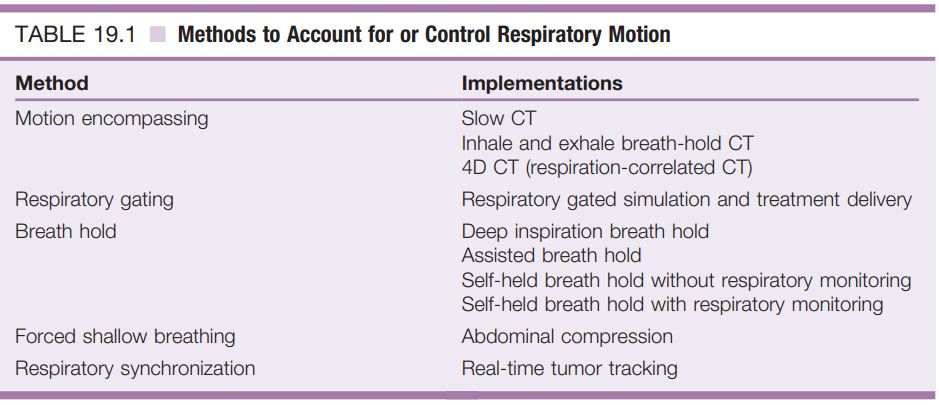
\includegraphics[width=0.8\textwidth]{Imagens/tecnicasRespiratorio.JPG}
		}%
		\caption{Métodos para considerar ou controlar o movimento respiratório.}
		\label{fig:tecnicasRespiratorio}
	\end{figure}

	Cada um desses métodos tem pontos fortes e fracos e graus variados de complexidade. Independentemente do método selecionado, existem alguns problemas comuns:

	\begin{enumerate}[label=\textcolor{CarnationPink}{(\roman*)}]
		\item O método deve passar por comissionamento rigoroso e garantia de qualidade (QA) contínua.
		\item O movimento respiratório deve ser considerado durante a simulação.
		\item As margens de planejamento devem ser identificadas.
		\item O movimento respiratório durante a simulação deve refletir com precisão o movimento respiratório durante o tratamento (por exemplo, se forem usados dispositivos de controle de movimento, eles devem ser idênticos e ter as mesmas configurações durante o tratamento).
		\item O paciente deve ser capaz de cumprir a estratégia de gerenciamento de movimento.
		\item Pode haver uma interação adicional com relação à administração de radioterapia de intensidade modulada (IMRT).
		\item O gerenciamento de movimento exigirá mais recursos e pode resultar em tempos de tratamento mais longos.
		\item O movimento do tecido alvo e normal não se limita ao pulmão. As estruturas abdominais também são afetadas.
		\item Todas as modalidades de imagem são afetadas pelo movimento respiratório.
		\item A movimentação do tumor não é a única fonte de incerteza e pode nem ser a maior.
	\end{enumerate}

	O objetivo final é garantir que a dose de radiação seja entregue com a máxima precisão aos alvos, levando em consideração o movimento respiratório, ao mesmo tempo em que se minimiza a dose nos tecidos saudáveis circundantes. Isso não apenas aumenta a eficácia do tratamento, mas também reduz as complicações e os efeitos colaterais associados à radiação nos tecidos normais. O contínuo desenvolvimento de métodos de controle e gerenciamento do movimento respiratório é fundamental para aprimorar a qualidade e a segurança da radioterapia.

\section{Medida do Movimento Respiratório}

	O ciclo respiratório é um processo complexo que envolve a contração e relaxamento de vários músculos respiratórios para permitir a entrada e saída de ar dos pulmões. Durante a inspiração, o diafragma se contrai e os músculos intercostais se contraem, puxando o diafragma para baixo e as costelas para cima e para fora. Isso aumenta o volume da cavidade torácica, criando um gradiente de pressão negativa que permite a entrada de ar nos pulmões. Ao mesmo tempo, o abdômen se desloca para baixo e para frente devido ao movimento descendente do diafragma, contribuindo para a expansão da cavidade torácica. Durante a expiração, os músculos respiratórios relaxam, o diafragma volta à sua posição relaxada e as costelas se movem para baixo e para dentro, diminuindo o volume da cavidade torácica e empurrando o ar para fora dos pulmões.

	A amplitude e a profundidade da respiração podem variar de acordo com as necessidades do corpo e o nível de atividade física. Uma inspiração superficial é caracterizada por um volume menor de ar inspirado, enquanto uma inspiração profunda envolve um maior volume de ar inspirado. A respiração normal ocorre em um nível intermediário, em que o volume de ar inspirado é suficiente para atender às demandas do corpo em repouso ou em atividades leves. Durante a respiração normal, o volume pulmonar pode aumentar de 10\% a 25\% em relação ao volume pulmonar no final da expiração.

	A medição e o gerenciamento do movimento respiratório são componentes cruciais na radioterapia, especialmente quando se lida com o movimento dos órgãos-alvo e das estruturas críticas durante o planejamento e a entrega do tratamento. Existem várias abordagens para medir o movimento respiratório. A observação direta da estrutura de interesse pode ser realizada visualmente, mas isso pode ser limitado em termos de precisão e praticidade. Uma alternativa é o uso de marcadores fiduciais implantados, que são dispositivos colocados dentro do corpo do paciente e podem ser detectados por meio de técnicas de imagem. Esses marcadores fornecem informações precisas sobre o movimento do alvo durante a respiração.

	Outra abordagem é o uso de estruturas substitutas, como o diafragma ou a parede torácica, para estimar o movimento respiratório. Essas estruturas podem ser monitoradas por meio de técnicas de imageamento ou sensores externos, como sensores de pressão colocados na superfície do corpo do paciente. Esses métodos são mais convenientes e não invasivos em comparação com a implantação de marcadores fiduciais, mas podem ter limitações em termos de precisão e correlação com o movimento do alvo real.

	Além da medição do movimento respiratório, é importante desenvolver estratégias de gerenciamento do movimento para lidar com as variações individuais dos pacientes e as variações no ciclo respiratório ao longo do tempo. Cada paciente possui padrões de respiração únicos, e mesmo um único paciente pode ter variações no ciclo respiratório durante uma sessão de tratamento ou de um dia para o outro. A \ref{fig:gmrVariacoesNoCiclo} mostra um exemplo de padrões respiratórios para um paciente durante um período de minutos. A respiração do paciente é regular na primeira sessão (painel A), mas torna-se mais irregular na segunda sessão (painel B).

	\begin{figure}[h]
		\centering
		\fcolorbox{DarkTurquoise}{white}{%
			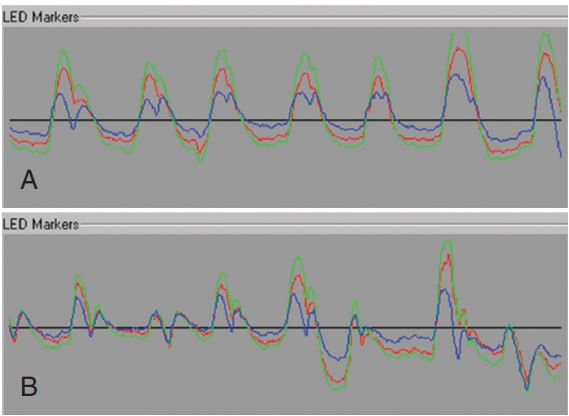
\includegraphics[width=0.7\textwidth]{Imagens/gmrVariacoesNoCiclo.JPG}
		}%
		\caption{Variação do ciclo respiratório de um único paciente em duas sessões diferentes. Cada cor representa um dos três marcadores externos usados..}
		\label{fig:gmrVariacoesNoCiclo}
	\end{figure}

	O treinamento respiratório e o feedback audiovisual podem ser utilizados para ajudar a regularizar o ciclo respiratório e garantir uma respiração mais consistente e previsível durante o tratamento. Isso pode envolver a exibição da informação do ciclo respiratório em tempo real para o paciente, juntamente com orientações visuais para ajudar o paciente a ajustar a amplitude e o ritmo da respiração de acordo com o desejado.

	O movimento dos órgãos durante o ciclo respiratório é um fator importante a ser considerado no planejamento e na entrega da radioterapia. Para compreender o alcance desse movimento, vários estudos têm sido realizados utilizando diferentes modalidades de imagem para medir o movimento dos órgãos, incluindo o pulmão. O relatório AAPM TG-76 fornece uma compilação de dados sobre o movimento observado no pulmão, com base em estudos publicados até cerca de 2006.

	A Tabela 1 no relatório apresenta referências específicas para cada modalidade de imagem utilizada na medição do movimento dos órgãos. Essas modalidades incluem tomografia computadorizada (CT), ressonância magnética (RM), fluoroscopia, entre outras. A Tabela 2, por sua vez, apresenta uma amostra do movimento observado no pulmão a partir desses estudos, que é adaptado e mostrado na \ref{fig:gmrVariacaoPulmao}.

	\begin{figure}[h]
		\centering
		\fcolorbox{DarkTurquoise}{white}{%
			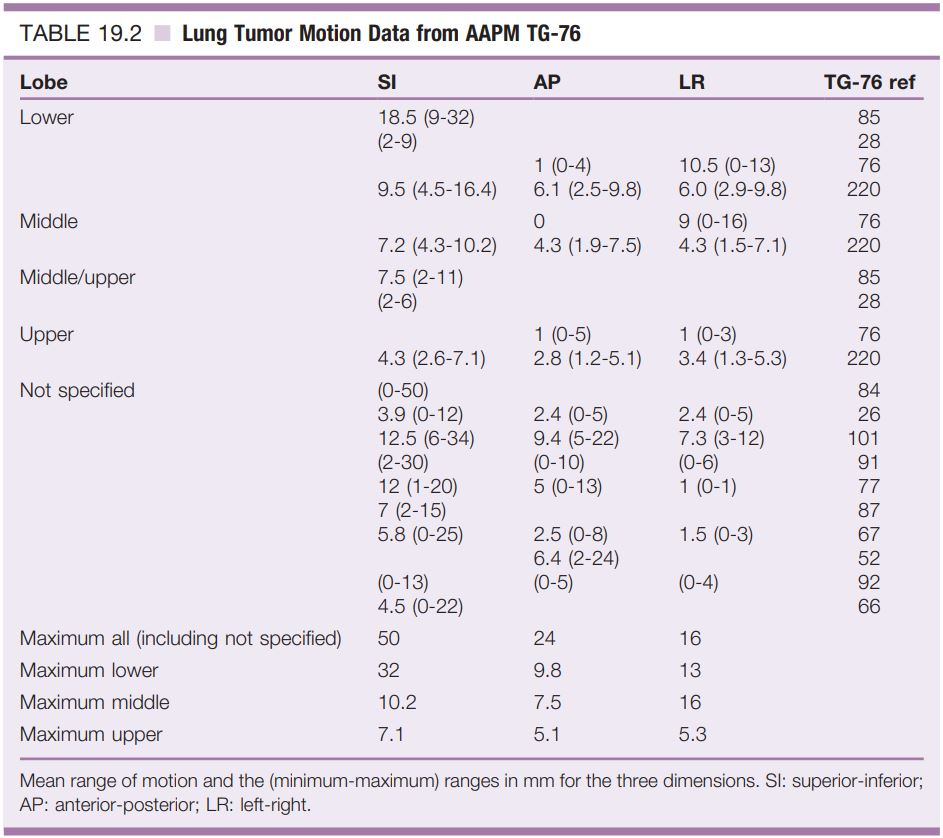
\includegraphics[width=0.7\textwidth]{Imagens/gmrVariacaoPulmao.JPG}
		}%
		\caption{Dados de movimento do tumor pulmonar do AAPM TG-76.}
		\label{fig:gmrVariacaoPulmao}
	\end{figure}

	Os dados mostram que o movimento do pulmão durante a respiração pode ser bastante variável. A amplitude do movimento pode chegar a até 50 mm em alguns pacientes, o que demonstra a importância de considerar o movimento respiratório no planejamento do tratamento. Além disso, observa-se que a amplitude máxima do movimento varia de acordo com o lobo do pulmão. O lobo inferior apresenta a maior amplitude de movimento, seguido pelo lobo médio e, por fim, pelo lobo superior. Essa diferença pode ser atribuída à localização anatômica desses lobos em relação ao diafragma.

	Outra observação é que o movimento apresenta diferentes amplitudes nas direções superior-inferior (SI), anterior-posterior (AP) e esquerda-direita (LR). A direção SI apresenta a maior amplitude de movimento, seguida pela direção AP e, por fim, pela direção LR. Essa distribuição do movimento pode ser explicada pelas características anatômicas e biomecânicas do sistema respiratório.

	No entanto, é importante ressaltar que esses dados são baseados em estudos limitados e representam apenas uma amostra da variação do movimento observado no pulmão. Cada paciente é único, e o movimento dos órgãos pode variar consideravelmente de um indivíduo para outro. Portanto, é necessário uma avaliação individualizada do movimento respiratório de cada paciente durante o planejamento do tratamento radioterápico, a fim de garantir uma entrega precisa da radiação aos alvos e minimizar a dose nos tecidos saudáveis circundantes.

	Vários estudos demonstraram a presença de histerese nas trajetórias dos tumores. Isso significa que a trajetória durante a inspiração é diferente da trajetória durante a expiração e que a amplitude máxima de movimento pode não ser observada durante a inspiração completa, como mostra a \ref{fig:gmrVariacaoTrajetoriaBronq}.Isso terá um impacto nas estratégias de gerenciamento do movimento.

	\begin{figure}[h]
		\centering
		\fcolorbox{DarkTurquoise}{white}{%
			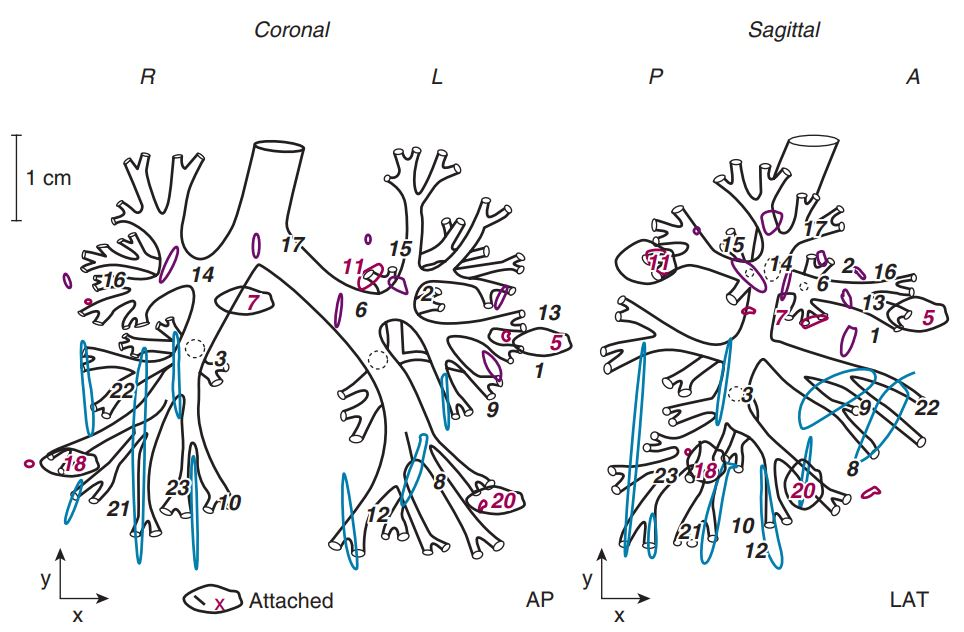
\includegraphics[width=0.7\textwidth]{Imagens/gmrVariacaoTrajetoriaBronq.JPG}
		}%
		\caption{Variação da trajetória do tumor durante a inspiração e expiração, histerese. Cada número indica um paciente diferente estudado.}
		\label{fig:gmrVariacaoTrajetoriaBronq}
	\end{figure}

	A histerese é um fenômeno em que a resposta de um sistema não é instantânea e apresenta uma defasagem em relação ao estímulo aplicado. No contexto do movimento respiratório, a histerese se refere à diferença nas trajetórias do tumor entre a fase de inspiração e a fase de expiração. As propriedades elásticas dos tecidos, a interação entre os órgãos e a variação da pressão intratorácica podem contribuir para esse efeito.

	A presença de histerese nas trajetórias dos tumores implica que a amplitude máxima de movimento do tumor pode não ser alcançada durante a inspiração completa. Isso significa que, ao planejar e entregar a radioterapia, é importante considerar não apenas a amplitude de movimento máxima observada, mas também as diferenças nas trajetórias durante a inspiração e a expiração. Estratégias de gerenciamento do movimento devem levar em conta essa variabilidade para garantir uma entrega precisa da radiação ao longo do ciclo respiratório.

	O reconhecimento da histerese nas trajetórias dos tumores tem levado ao desenvolvimento de abordagens mais sofisticadas de gerenciamento do movimento respiratório. Isso pode envolver o uso de técnicas de imageamento 4D para capturar a variabilidade temporal do movimento, a aplicação de algoritmos de previsão para estimar as trajetórias futuras do tumor e a adaptação do tratamento com base nas informações em tempo real durante a entrega da radiação.

	O relatório AAPM TG-76 afirma que, em geral, o movimento dos órgãos abdominais ocorre predominantemente na direção superior-inferior (SI), com uma amplitude de movimento de até 2 mm nas direções anterior-posterior (AP) e esquerda-direita (LR). No entanto, essa afirmação foi baseada em dados iniciais de tomografia computadorizada 4D e provavelmente não é correta. O relatório também menciona que, em alguns indivíduos, os rins podem apresentar movimentos mais complexos.

	É importante ressaltar que o movimento dos órgãos abdominais pode variar consideravelmente de um paciente para outro e até mesmo em diferentes situações clínicas. A amplitude e a direção do movimento podem ser influenciadas por vários fatores, como a anatomia individual, a posição do paciente, a respiração e o estado de preenchimento dos órgãos.

	Estudos mais recentes têm demonstrado que o movimento dos órgãos abdominais pode ser mais complexo do que inicialmente relatado. Por exemplo, o movimento dos rins pode apresentar variações significativas e pode ser influenciado pela respiração, pelo estado de preenchimento da bexiga e por fatores individuais. Além disso, outros órgãos abdominais, como o fígado, o pâncreas e os órgãos gastrointestinais, também podem exibir movimentos significativos durante o ciclo respiratório.

\section{Tracking do Ciclo Respiratório Através de Substitutos Anatômicos}

	
	Com a tecnologia atualmente disponível, não é viável observar diretamente o movimento do tumor ou o movimento respiratório durante o tratamento radioterápico (ou mesmo durante a realização da varredura de simulação). Portanto, é necessário utilizar substitutos anatômicos que possam indicar o ciclo respiratório. Esses substitutos podem incluir o deslocamento da parede torácica e abdominal, que é observado através da alteração do contorno externo do paciente. Para isso, é colocado um marcador na superfície do paciente e esse marcador é rastreado por meio de uma câmera (infravermelha ou de luz visível), um cinto sensível à pressão ao redor do abdômen do paciente, ou através da captura direta e rastreamento da superfície do paciente usando câmeras estereoscópicas ou lasers. Além disso, a espirometria e a detecção do diafragma também têm sido utilizadas nesse contexto. A \ref{fig:gmrTracking} apresenta algumas tecnologias disponíveis para serem utilizadas no rastreamento do ciclo respiratório.

	\begin{figure}[h]
		\centering
		\fcolorbox{DarkTurquoise}{white}{%
			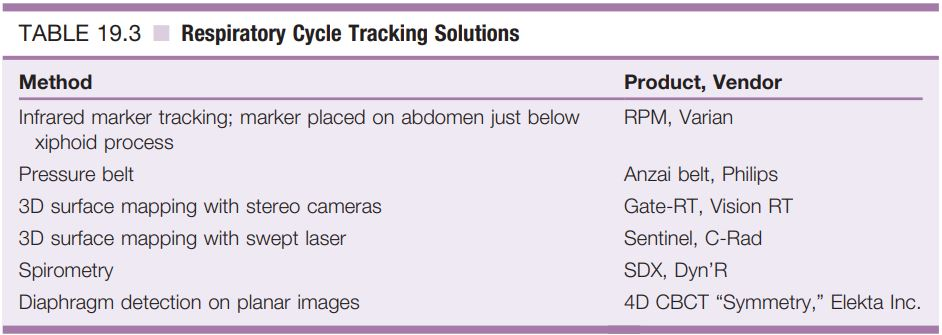
\includegraphics[width=0.8\textwidth]{Imagens/gmrTracking.JPG}
		}%
		\caption{Soluções de monitoramento do ciclo respiratório.}
		\label{fig:gmrTracking}
	\end{figure}

	Essas técnicas permitem uma estimativa indireta do movimento respiratório ao observar as alterações externas no contorno do paciente. Ao analisar o deslocamento da parede torácica e abdominal, é possível inferir o movimento interno dos órgãos durante a respiração. A espirometria, que envolve a medição do volume e do fluxo respiratório, e a detecção do diafragma por meio de técnicas de imagem ou sensores, também fornecem informações valiosas sobre o ciclo respiratório do paciente.

	Com qualquer um desses métodos, não se pode presumir que exista uma relação direta entre o movimento da anatomia substituta e o tumor em si, nem que eles estejam sincronizados. O relatório AAPM TG-76 descreve diversos estudos nos quais foi observada uma diferença de fase de 0,5 a 1 segundo. Além disso, verificou-se que a diferença de fase entre a anatomia substituta e o próprio tumor pode variar ao longo do tratamento. Portanto, o uso de qualquer substituto introduzirá incertezas.

	É importante ressaltar que, ao utilizar um substituto anatômico para estimar o movimento do tumor, não se pode ter certeza de que o movimento do substituto está perfeitamente alinhado com o movimento real do tumor. O deslocamento de fase, ou a diferença no tempo entre os movimentos do substituto e do tumor, pode variar consideravelmente. Além disso, ao longo do tratamento, essa diferença de fase pode mudar, o que aumenta ainda mais a incerteza.

	Portanto, é necessário ter em mente que o uso de um substituto anatômico introduzirá uma certa quantidade de incerteza na estimativa do movimento do tumor. Essa incerteza deve ser considerada no planejamento e na execução do tratamento radioterápico, a fim de garantir a precisão e a eficácia do tratamento. Estratégias adicionais, como a verificação regular do alinhamento do substituto com o tumor e a adaptação do plano de tratamento com base nas variações observadas, podem ajudar a minimizar a incerteza e melhorar a precisão do tratamento radioterápico.

\section{Abrangência de Movimento}

	Como apresentado na \ref{fig:tecnicasRespiratorio} existem várias maneiras de visualizar a extensão do movimento e, assim, delimitar um volume que englobe toda essa extensão de movimento.

\subsubsection*{4D CT/ CT Correlacionada à Respiração}

	A TC 4D é uma técnica avançada de imagem que permite a visualização e a avaliação do movimento dos tecidos ao longo do ciclo respiratório. Ela é chamada de "4D" porque adiciona uma dimensão extra (tempo) às imagens de TC tradicionais, que são 3D.

	A aquisição da TC 4D é realizada com o paciente em posição de tratamento, geralmente na posição de supino (deitado de costas). Durante o exame, são adquiridas imagens sequenciais em diferentes fases do ciclo respiratório. Essas imagens são posteriormente correlacionadas com base em informações fornecidas pelos sensores de respiração ou pelos marcadores colocados no paciente. Esse processo permite que cada imagem seja associada a uma fase específica da respiração. Ao visualizar as imagens adquiridas, é possível observar o movimento dos tecidos em 3D ao longo do tempo, criando uma espécie de "filme" que mostra a variação da posição dos órgãos e do tumor durante o ciclo respiratório.

	A TC 4D foi introduzida pela primeira vez em 2003, em um artigo que descreveu a técnica e suas aplicações clínicas. Desde então, ela tem sido amplamente adotada pelos fabricantes de equipamentos de radioterapia e está disponível em muitas clínicas ao redor do mundo. 

	Para obter conjuntos de dados de imagem 4D, é necessário sincronizar as projeções adquiridas durante a tomografia computadorizada (TC) com o ponto correspondente no ciclo respiratório. Isso é feito por meio da obtenção de um traçado respiratório que registra as variações respiratórias do paciente durante a aquisição dos dados de TC.

	Existem duas abordagens principais para realizar a classificação respiratória: retrospectiva e prospectiva. Na classificação retrospectiva, o traçado respiratório é adquirido simultaneamente com as projeções de TC. Posteriormente, cada projeção é correlacionada com um ponto específico no ciclo respiratório com base nas informações do traçado respiratório. Isso permite agrupar as projeções em compartimentos ou bins correspondentes a diferentes fases da respiração. Geralmente, são usados cerca de 10 compartimentos por ciclo respiratório. Em seguida, as projeções são reconstruídas em conjuntos de dados 3D correspondentes a cada compartimento.

	Com base nesses conjuntos de dados 3D para cada compartimento respiratório, é possível percorrer as imagens e observar o movimento 4D dos tecidos ao longo do ciclo respiratório. Essa visualização abrange toda a amplitude do movimento respiratório, permitindo uma compreensão detalhada do comportamento do tumor e dos órgãos durante a respiração.

	No entanto, a delimitação (contouring) manual do tumor e das estruturas relevantes em cada conjunto de dados 3D seria um trabalho demorado, pois haveria aproximadamente 10 conjuntos de dados. Para facilitar esse processo, os fabricantes desenvolveram algoritmos que propagam os contornos desenhados em um conjunto para os demais conjuntos. Isso reduz significativamente o tempo necessário para realizar a delimitação manual em todos os conjuntos.

	É importante ressaltar que, apesar da vantagem de ter imagens nítidas em cada compartimento respiratório, as imagens de TC 4D geralmente apresentam mais ruído em comparação com uma varredura helicoidal padrão. Isso ocorre porque os protocolos de aquisição de TC 4D costumam reduzir a corrente (mA) para limitar a dose de radiação administrada ao paciente.

	Por outro lado, na classificação prospectiva, as projeções são adquiridas em momentos específicos e definidos do ciclo respiratório. Isso requer a sincronização precisa entre o sistema de aquisição de imagens e o ciclo respiratório do paciente. Dessa forma, cada projeção é diretamente associada a um ponto específico no ciclo respiratório, eliminando a necessidade de classificação retrospectiva.

	A determinação dos compartimentos respiratórios é um aspecto crucial na classificação dos dados de imagem 4D, e existem diferentes abordagens para essa tarefa. Duas abordagens comuns são o agrupamento baseado na fase e o agrupamento baseado na amplitude respiratória. A \ref{fig:gmrAmplitudeDeFase} mostra a diferença entre estas duas abordagens. No agrupamento baseado na fase, os compartimentos são definidos com base na relação temporal das projeções de TC com o ciclo respiratório. Por exemplo, pode-se dividir o ciclo respiratório em um número fixo de fases, como 10 compartimentos igualmente espaçados. Cada projeção é então atribuída ao compartimento correspondente com base em sua relação temporal com o ciclo respiratório. Já no agrupamento baseado na amplitude respiratória, os compartimentos são determinados com base na fração da amplitude máxima do movimento respiratório. Por exemplo, pode-se definir compartimentos correspondentes a frações específicas da amplitude respiratória, como 10 compartimentos igualmente espaçados em termos de frações da amplitude máxima. Cada projeção é atribuída ao compartimento que representa a fração de amplitude correspondente. 

	\begin{figure}[h]
		\centering
		\fcolorbox{DarkTurquoise}{white}{%
			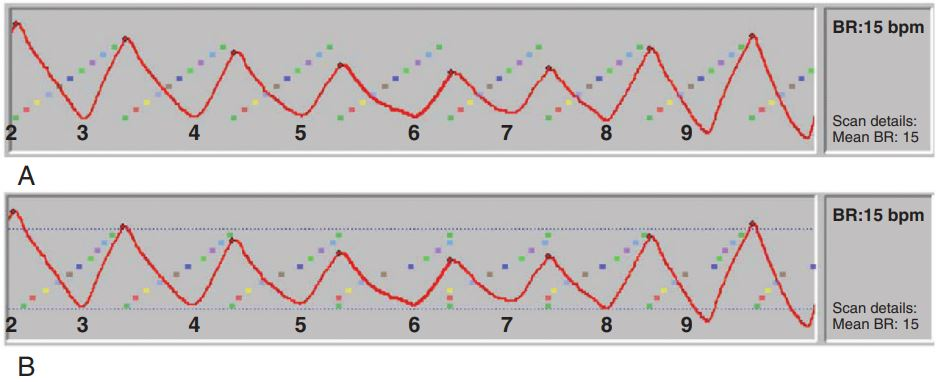
\includegraphics[width=0.8\textwidth]{Imagens/gmrAmplitudeDeFase.JPG}
		}%
		\caption{Classificação do ciclo respiratório baseado em amplitude versus fase.}
		\label{fig:gmrAmplitudeDeFase}
	\end{figure}


	O algoritmo utilizado para determinar o melhor método de agrupamento depende da observação de irregularidades na amplitude e/ou no padrão do ciclo respiratório. Por exemplo, se houver irregularidades evidentes na amplitude, como variações abruptas ou inconsistentes, pode ser preferível usar o agrupamento baseado na fase. Por outro lado, se houver irregularidades mais pronunciadas no padrão temporal, como alterações na duração ou na forma do ciclo respiratório, o agrupamento baseado na amplitude pode ser mais adequado. 

	Além da tomografia computadorizada (TC), outras modalidades de imagem, como a CBCT, PET e RM, também podem ser usadas para adquirir imagens 4D. Essas técnicas permitem a visualização do movimento dos tecidos ao longo do ciclo respiratório e são especialmente úteis no planejamento e na entrega de tratamentos de radioterapia. No caso da CBCT 4D, a aquisição é realizada por meio do equipamento de CBCT, que captura uma série de imagens planares em diferentes fases da respiração. Durante esse processo, o software de aquisição de imagens automaticamente detecta a posição do diafragma, que é usado como uma estrutura de referência para correlacionar as imagens com o ciclo respiratório. O diafragma é uma estrutura muscular localizada abaixo dos pulmões e é um indicador confiável do movimento respiratório. Ao detectar a posição do diafragma nas imagens planares adquiridas durante o CBCT, é possível determinar a fase do ciclo respiratório correspondente a cada imagem.


\subsubsection*{CT Lenta}

	A técnica de CT slow é uma alternativa para a aquisição de imagens 4D em que o scanner de TC é operado em uma velocidade de rotação reduzida ou são adquiridas múltiplas varreduras que são posteriormente combinadas. Essa abordagem permite coletar dados durante vários ciclos respiratórios, geralmente em torno de 5 segundos, abrangendo toda a amplitude do movimento respiratório na região de interesse. 

	Ao executar o scanner de CT em uma taxa de rotação lenta ou adquirir várias varreduras, é possível capturar imagens em diferentes fases do ciclo respiratório. Essas imagens são então combinadas ou médias para gerar uma imagem representativa do estado médio do paciente. Essa técnica é especialmente útil para cálculos precisos de dose, uma vez que representa uma condição média do paciente ao longo do ciclo respiratório.

	No entanto, uma desvantagem do CT slow é que as imagens resultantes são borradas, devido à integração temporal dos dados em várias fases respiratórias. Essa borragem pode dificultar a visualização e a delimitação das estruturas de interesse, tornando a interpretação e o planejamento do tratamento mais desafiadores. Portanto, é necessário ter cuidado ao utilizar imagens de CT slow para delineação precisa das estruturas anatômicas.

	Uma alternativa é a criação de uma varredura de projeção de intensidade média, que combina diferentes fases respiratórias de uma varredura de CT 4D. Essa técnica permite gerar uma imagem que representa a média das intensidades dos pixels ao longo do ciclo respiratório, fornecendo uma visualização simplificada das estruturas em movimento.

	A escolha entre a técnica de CT slow e a aquisição de imagens 4D depende das necessidades e objetivos específicos de cada caso. O CT slow é útil para cálculos de dose mais precisos, mas pode apresentar desafios na visualização das estruturas de interesse. Por outro lado, a aquisição de imagens 4D fornece uma representação mais detalhada do movimento respiratório, permitindo um planejamento mais refinado do tratamento radioterápico.


\section{Limitação do Movimento Respiratório}

	As técnicas de respiração superficial forçada são utilizadas para minimizar o movimento do diafragma durante a aquisição de imagens ou a administração de tratamentos de radioterapia. O movimento do diafragma pode afetar a precisão do tratamento, especialmente quando a área de interesse está localizada em regiões afetadas pela respiração, como o tórax e o abdômen. Diversos dispositivos e métodos foram desenvolvidos para aplicar pressão reprodutível no abdômen do paciente e limitar o movimento do diafragma. Esses métodos geralmente envolvem a aplicação de pressão sobre o abdômen e o tórax, com o objetivo de reduzir o movimento respiratório e melhorar a precisão do tratamento.

	Alguns sistemas, como o sistema de estrutura corporal e o sistema Body Fix, utilizam placas de compressão abdominal ou uma almofada a vácuo que se estende ao longo do corpo do paciente. Esses dispositivos são projetados para fornecer uma superfície de apoio estável e aplicar pressão uniforme sobre o abdômen e o tórax, limitando assim o movimento do diafragma durante a respiração. Outros métodos envolvem o uso de cintos de velcro que são envoltos ao redor do abdômen do paciente com um comprimento consistente. A pressão é aplicada por meio de uma bolsa inflável de ar, semelhante a um manguito de pressão arterial. A pressão na bolsa é ajustada e monitorada durante o tratamento para garantir que o movimento respiratório seja adequadamente limitado.

	Ao aplicar qualquer método para limitar a respiração, é necessário realizar um processo de ajuste para encontrar a pressão ideal que reduza o movimento do diafragma para as faixas desejáveis, geralmente de 5 a 10 mm. É importante equilibrar a redução do movimento com o conforto do paciente, pois o aumento excessivo da pressão pode causar desconforto e, paradoxalmente, aumentar o movimento respiratório. Além disso, ao utilizar dispositivos para limitar a respiração, é necessário considerar se os feixes de tratamento de radioterapia passarão através desses dispositivos. A geometria do tratamento e a localização dos dispositivos devem ser cuidadosamente planejadas para garantir que os feixes alcancem a área de tratamento com a precisão adequada.

\section{Gating Respiratório}

	O gating respiratório é uma técnica que envolve o planejamento e a administração de feixes de tratamento de radioterapia em sincronia com o ciclo respiratório do paciente. Durante a aquisição de imagens e a entrega do tratamento, o paciente respira normalmente, sem a necessidade de técnicas de respiração superficial forçada ou restrições na respiração. O objetivo do gating é administrar o feixe de tratamento somente durante um segmento específico do ciclo respiratório, chamado de "gate". A determinação da posição e da largura do gate é importante para garantir que o movimento do tumor esteja restrito a um limite específico durante a fase de entrega do tratamento. Isso é geralmente feito observando a quantidade de movimento do tumor e ajustando o gate para abranger somente o intervalo de movimento aceitável, que é tipicamente definido em torno de 5 mm.

	O gating respiratório pode ser realizado usando fluoroscopia, que fornece imagens em tempo real do movimento do tumor durante a respiração, ou através de uma varredura completa de CT 4D, que permite a visualização e a classificação das imagens em diferentes fases respiratórias. A porcentagem de tempo em que o sinal respiratório está dentro do gate é chamada de "duty cycle" e geralmente é de cerca de 30\% quando o gating ocorre na parte final da expiração do ciclo respiratório. Isso significa que os tempos de entrega do feixe de tratamento com gating são geralmente pelo menos 3 vezes mais longos do que os tratamentos convencionais. A vantagem desse método é que ele permite volumes de tratamento menores, pois o tratamento é entregue apenas em uma faixa limitada do movimento do tumor.

	No entanto, é importante observar que o gating respiratório depende do uso de um marcador anatômico substituto para rastrear o ciclo respiratório. Esse marcador pode ser um bloco colocado no abdômen do paciente, que é usado para monitorar o movimento respiratório e ajustar o gating em conformidade. A precisão do gating depende da consistência da relação de fase entre a posição do marcador substituto e a do tumor ao longo do tempo. Estudos recentes mostraram que essa relação de fase pode variar ao longo do tratamento, o que pode levar a variações na posição do tumor durante as sessões de radioterapia, mesmo quando a mesma janela de gating é usada. Essas descobertas, juntamente com outras considerações, levaram alguns centros a interromper o uso do gating respiratório em determinados casos ou buscar aprimoramentos técnicos para melhorar sua precisão.

\section{Técnicas de Retenção da Respiração (Breath-Hold)}

	As técnicas de retenção respiratória são utilizadas para minimizar o movimento de um tumor durante a administração do tratamento de radioterapia, "congelando" o movimento do tumor enquanto o feixe de tratamento está ligado. Isso pode ser especialmente benéfico no caso de tumores localizados em áreas sensíveis a movimentos respiratórios, como o pulmão. Neste caso, realizar apneias respiratórias com inspiração completa oferece uma vantagem dosimétrica adicional. Durante a inspiração completa, mais tecido pulmonar saudável é expandido, afastando-o da região de alta dose, o que ajuda a reduzir a dose recebida pelos tecidos saudáveis circundantes.

	No entanto, realizar apneias respiratórias é um processo complexo e desafiador para muitos pacientes. Alguns pacientes podem ter dificuldades em cumprir as apneias por questões sociais, de idioma ou de saúde. Isso é especialmente relevante no caso de pacientes com câncer de pulmão, que podem ter uma função pulmonar comprometida ou outros problemas respiratórios. É importante avaliar os pacientes previamente para determinar se eles são candidatos adequados para técnicas de apneia respiratória. Isso deve ser feito durante a fase de simulação do tratamento, para garantir que o equipamento e a técnica utilizados sejam os mesmos durante o tratamento real.

	O feedback audiovisual (AV) é uma abordagem comum para ajudar os pacientes a realizar as apneias respiratórias corretamente. Isso pode ser feito usando óculos de vídeo ou dispositivos eletrônicos, como Kindles ou iPads (quando o VisionRT está disponível), que fornecem ao paciente uma referência visual para ajudar a manter a posição ideal durante as apneias. Algumas instituições também estão explorando a abordagem combinada de apneia respiratória/gating, na qual o paciente executa apneias respiratórias que se ajustam a uma janela de gating específica. Essa abordagem busca combinar os benefícios da apneia respiratória e do gating para melhorar a precisão do tratamento. No entanto, existem desafios técnicos e clínicos associados a essa abordagem, e sua eficácia e viabilidade ainda estão sendo estudadas.

\subsection*{Inspiração Profunda}

	A técnica de retenção inspiratória profunda, também conhecida como "deep inspiration breath hold" (DIBH), é frequentemente utilizada no tratamento de câncer de mama esquerda para proteger os órgãos em risco, como o pulmão e o coração, da exposição à radiação. Durante a inspiração profunda, a expansão do pulmão e a afastamento do coração da área de tratamento ajudam a reduzir a dose de radiação recebida por esses órgãos críticos. Uma das vantagens da técnica de DIBH é que ela torna o volume e o posicionamento do pulmão mais reproduzíveis, uma vez que o paciente é levado a um volume tidal pulmonar\footnote{O volume tidal pulmonar refere-se à quantidade de ar que entra e sai dos pulmões durante uma respiração normal} quase máximo durante cada apneia respiratória. Isso significa que, a cada inspiração profunda, o pulmão atinge um estado semelhante e previsível, permitindo que o planejamento e a administração do tratamento sejam mais precisos.

	No entanto, a técnica de DIBH requer um paciente cooperativo e capaz de participar ativamente do processo. O paciente é instruído a realizar uma inspiração profunda e a manter essa posição durante a administração do feixe de tratamento. Para ajudar o paciente a alcançar consistentemente o nível adequado de inspiração, é comum fornecer feedback audiovisual (AV). O feedback AV pode ser fornecido por meio de soluções de mapeamento tridimensional da superfície corporal, como o Align RT da Vision RT. Esses sistemas monitoram continuamente o nível de inspiração do paciente e fornecem informações visuais em tempo real, permitindo que o paciente ajuste sua respiração para atingir a posição correta de inspiração.

	Estudos demonstraram que o uso de soluções de mapeamento tridimensional da superfície corporal, como o Align RT, é uma abordagem superior para monitorar o nível de inspiração durante a técnica de DIBH. Esses sistemas oferecem maior precisão e reprodutibilidade em comparação com métodos tradicionais, como a avaliação visual ou medições manuais.

\subsection*{Breath-Hold Assistida}

	O método de apneia respiratória assistida, foi desenvolvido no Hospital William Beaumont e agora é comercializado como Active Breathing Control (ABC) pela Elekta. Este método foi desenvolvido para auxiliar os pacientes durante as apneias respiratórias e garantir uma respiração controlada e precisa. O ABC consiste em um dispositivo que combina um espirômetro digital para medir o volume respiratório e uma válvula balão que pode ser fechada para suspender a respiração em um ponto específico do ciclo respiratório.

	Durante o uso do ABC, o paciente realiza a respiração normalmente, enquanto o espirômetro digital monitora o volume respiratório. Quando o ponto desejado do ciclo respiratório é alcançado, a válvula balão é fechada, forçando o paciente a fazer uma apneia respiratória controlada. Para garantir uma apneia respiratória efetiva, é importante que haja uma vedação adequada no bocal do dispositivo e que um clipe nasal seja usado para evitar vazamentos de ar. Isso garante que o ar não escape durante a apneia respiratória e ajuda a manter a estabilidade do volume pulmonar durante o tratamento.

	No entanto, existem dados mistos sobre o desempenho do ABC em comparação com as técnicas de apneia voluntária, nas quais o paciente realiza apneias respiratórias sem o uso de dispositivos auxiliares. Um estudo randomizado mostrou diferenças insignificantes entre as abordagens, mas o estudo incluiu apenas um número limitado de pacientes.

\subsection*{Breath-Hold Autônoma}

	A técnica de autoapneia respiratória é uma abordagem na qual o paciente realiza uma apneia voluntária durante a administração do tratamento de radioterapia. Essa técnica pode ser realizada com ou sem monitoramento respiratório adicional. 

	Quando a autoapneia é feita sem monitoramento, o paciente é instruído a segurar a respiração em um ponto específico do ciclo respiratório, geralmente na inspiração profunda. O paciente utiliza um dispositivo, como um interruptor ou um dispositivo de segurança, para controlar o início e o término da apneia respiratória. Ao acionar o dispositivo, o terapeuta pode ligar o feixe de tratamento, e ao liberá-lo, o feixe é desligado. É importante ressaltar que essa técnica requer um paciente altamente cooperativo e capaz de realizar a apneia respiratória com precisão. A dependência do paciente torna esse método menos ideal em comparação com outras técnicas de apneia respiratória, que podem utilizar dispositivos de monitoramento mais avançados para garantir uma apneia respiratória precisa e consistente.

	Empresas como a Varian e a Elekta desenvolveram interfaces específicas para seus sistemas de tratamento de radioterapia, que podem ser utilizadas para implementar a técnica de autoapneia. A Varian atualmente oferece uma interface para linacs das séries C e superiores para implementar essa técnica. A Elekta também oferece uma interface de gating chamada "Response", que pode alcançar alguns desses objetivos. 

	Uma vantagem desse método é que, com o uso de taxas de dose mais altas nos linacs, a entrega do tratamento pode ser realizada de forma eficiente, com uma quantidade significativa de dose sendo entregue em um curto período de tempo. Por exemplo, um paciente típico pode manter a respiração por 10 a 15 segundos. A 600 unidades monitoras (UM)/min, 100 UM podem ser entregues em 10 segundos. A 400 UM/min, seriam necessários 15 segundos para entregar as mesmas 100 UM. A entrega completa do tratamento pode ser feita em 1 a 2 apneias respiratórias para feixes de ângulo fixo, tornando esse método razoavelmente eficiente. No entanto, é importante lembrar que a escolha da técnica de apneia respiratória, seja ela autoapneia ou outras formas de apneia, deve ser baseada na avaliação individual do paciente, nas características do tumor e nos recursos disponíveis na instituição de tratamento. 


	Em resumo, a técnica de autoapneia respiratória envolve uma apneia voluntária do paciente durante a administração do tratamento de radioterapia. Essa abordagem requer um paciente cooperativo e pode ser realizada com ou sem monitoramento respiratório adicional. Embora apresente desafios em termos de reprodutibilidade e dependência do paciente, a autoapneia pode ser uma opção viável, especialmente quando combinada com interfaces e sistemas de tratamento específicos.


\section{Movimento Respiratório e Planejamento de Tratamento}

\subsubsection*{Volumes Alvo}

	Ao utilizar técnicas de abrangência de movimento, como a radioterapia 4D, é importante criar um volume alvo interno (ITV) que capture adequadamente a amplitude completa do movimento do tumor durante o ciclo respiratório. O ITV é uma expansão do volume tumoral para incorporar o movimento observado durante a aquisição dos dados 4D. Para determinar o ITV, é comum adicionar uma margem de segurança ao volume máximo de movimento do tumor. Essa margem geralmente é de 5 mm para compensar possíveis variações e incertezas no movimento do tumor. A definição precisa do ITV é fundamental para garantir que o tratamento seja entregue com precisão ao tumor, mesmo considerando as flutuações respiratórias.

	Além disso, a análise dos dados 4D pode fornecer informações adicionais para o planejamento do tratamento. A projeção de intensidade máxima (MIP) é uma técnica em que a intensidade máxima de cada voxel em todas as fases do ciclo respiratório é relatada e usada para criar um conjunto de dados 3D. Isso resulta em uma representação visual em que os valores mais altos de densidade tumoral ao longo do ciclo respiratório são sobrepostos, delineando assim a amplitude total do movimento do tumor. Outra abordagem semelhante é registrar todas as fases do conjunto de dados 4D no sistema de planejamento e usar essas informações para contornar a extensão máxima do movimento. Isso envolve alinhar e combinar os contornos de todas as fases para obter uma representação abrangente do movimento do tumor.

	A projeção de intensidade mínima (MinIP) é o inverso da MIP, selecionando o valor mínimo de intensidade para cada voxel em todos os bins. Essa técnica pode ser útil para determinar a extensão do movimento de alvos localizados fora do pulmão, como o fígado. Ao destacar os valores de menor intensidade, a MinIP pode ajudar a identificar o alcance máximo do movimento desses alvos, auxiliando no planejamento do tratamento.

	A projeção de intensidade média (AIP) é uma técnica que calcula a intensidade média de cada voxel em todos os bins do conjunto de dados 4D. Essa média é então usada para criar um conjunto de dados 3D que representa uma visão geral do movimento do tumor ao longo do ciclo respiratório. A AIP é útil para fins de planejamento de dose, pois fornece uma representação mais realista da distribuição de dose que seria entregue ao tumor durante o tratamento. A tomografia computadorizada lenta (slow CT) é um método em que a aquisição do exame de tomografia computadorizada é realizada em um ritmo mais lento ou são adquiridos múltiplos exames e eles são então combinados em uma imagem. Essa abordagem resulta em uma imagem com menor borramento devido ao movimento respiratório em comparação com uma tomografia computadorizada convencional. A slow CT é considerada mais próxima da AIP em termos de representação do movimento do tumor e é preferida para o cálculo da dose de radiação, pois fornece uma base mais precisa para a entrega do tratamento.  

	Em resumo, a projeção de intensidade média (AIP) e a tomografia computadorizada lenta (slow CT) são técnicas preferidas para o cálculo da dose de radiação, pois fornecem uma representação mais precisa do movimento do tumor. A projeção de intensidade máxima (MIP) não deve ser usada para o cálculo da dose, pois distorce a inomogeneidade do corpo, enquanto a projeção de intensidade mínima (MinIP) pode ser útil para determinar o alcance máximo do movimento de alvos fora do pulmão. Essas técnicas de registro e contorno das diferentes fases do ciclo respiratório podem ser úteis para delinear a margem adequada para o ITV e auxiliar no planejamento preciso do tratamento. É importante ressaltar que, embora a MIP e o registro das fases do 4D sejam abordagens comuns, a escolha da técnica específica pode variar dependendo do sistema de planejamento utilizado e das preferências clínicas da equipe de tratamento. 

\subsubsection*{IMRT}

	A interação entre o movimento respiratório e as técnicas de entrega de IMRT tem sido uma área de estudo significativa na radioterapia. Durante a entrega de IMRT, as lâminas do MLC se movem dinamicamente para modular o feixe de radiação e moldar a dose de acordo com o contorno do alvo. No entanto, quando há movimento respiratório, pode haver uma interação complexa entre o movimento das lâminas e o movimento do tumor, o que pode resultar em variações indesejadas na distribuição de dose. Essa interação pode levar à formação de gradientes dentro do volume alvo, onde áreas de alta dose (hot spots) ou baixa dose (cold spots) podem ocorrer devido ao movimento das lâminas do MLC em relação ao movimento do tumor. Isso é particularmente relevante para alvos sujeitos a movimento respiratório, como tumores pulmonares.

	No entanto, estudos têm mostrado que, ao longo de um curso de tratamento completo, os erros de dose introduzidos pela interação entre o movimento das lâminas e o movimento do alvo tendem a se equilibrar. Isso significa que, apesar das variações temporais na distribuição de dose devido ao movimento, a dose média entregue ao longo do tratamento é geralmente consistente com a prescrição planejada. O AAPM TG-76 (Task Group 76) emitiu uma recomendação de cautela em relação ao uso de IMRT para alvos sujeitos a movimento respiratório, especialmente em tratamentos com poucas frações, como a SBRT. Essa recomendação destaca a importância de considerar cuidadosamente os efeitos do movimento respiratório nas técnicas de entrega de IMRT e nas estratégias de tratamento, e sugere a adoção de abordagens alternativas, como a radioterapia guiada por imagem (IGRT) com técnicas de controle de movimento mais avançadas.

\section{Imagem e Tracking Durante o Tratamento}

	O método ideal para administrar tratamentos a alvos que se movem durante o ciclo respiratório seria rastrear o movimento em tempo real. Isso permite uma maior redução do volume de tratamento, assim como no gating, mas sem a perda de eficiência exigida pelo ciclo de trabalho.O sistema CyberKnife é uma tecnologia avançada utilizada no tratamento de tumores que se movem durante o ciclo respiratório. Ele utiliza imagens fluoroscópicas cruzadas para detectar a posição do tumor quase em tempo real, o que permite um rastreamento preciso do movimento do tumor. Essas imagens são adquiridas em alta frequência, aproximadamente uma imagem por segundo, proporcionando uma visualização contínua do movimento do tumor. O linac (acelerador linear) é montado em um braço robótico que pode mover-se e sincronizar-se com o tumor, permitindo a administração precisa da radiação mesmo durante o movimento respiratório.

	Um aspecto importante do sistema CyberKnife é a capacidade de prever o movimento futuro do tumor. Isso se deve à amostragem temporal relativamente grosseira das imagens fluoroscópicas e ao tempo de atraso entre a detecção da posição do tumor e o momento em que o feixe de radiação é ativado. Para superar essas limitações, o sistema utiliza algoritmos avançados que levam em consideração o movimento anterior do tumor para prever seu movimento futuro. Essa capacidade de previsão permite que o linac esteja sempre sincronizado com o tumor, garantindo que a radiação seja direcionada com precisão ao alvo durante todo o ciclo respiratório.

	Inicialmente, a detecção da posição do tumor no sistema CyberKnife era feita por meio de um fiducial implantado no próprio tumor. No entanto, avanços recentes permitiram o desenvolvimento de métodos que não dependem mais do uso de fiduciais. Em vez disso, um colete com marcadores é utilizado para estabelecer uma representação em tempo real do movimento do tumor. Esses marcadores são detectados pelo sistema, permitindo o rastreamento e a correção contínua do movimento do tumor durante o tratamento.

	Além do sistema CyberKnife, outras abordagens têm sido exploradas para rastrear o movimento do tumor durante o tratamento. O sistema Calypso, por exemplo, utiliza um fiducial implantado e acompanha sua posição em tempo real por meio de sinais eletromagnéticos. Embora esse sistema seja amplamente utilizado no tratamento de câncer de próstata, pesquisas estão em andamento para implementar essa técnica em tumores de pulmão. Outra opção é o sistema Vero, que possui a capacidade de rastreamento em tempo real. Além disso, há o desenvolvimento de unidades de tratamento habilitadas para ressonância magnética, como o sistema ViewRay, que permitem a aquisição de imagens de ressonância magnética em tempo real durante o tratamento. Essa visualização em tempo real fornece informações adicionais para o planejamento e a administração precisa da radioterapia, eliminando a necessidade de fiduciais implantados.
	
	Essas abordagens de rastreamento em tempo real são importantes para garantir que a radiação seja entregue com precisão ao alvo, mesmo durante o movimento respiratório. Ao acompanhar e corrigir continuamente o movimento do tumor, esses sistemas permitem uma redução do volume de tratamento, resultando em uma melhor preservação dos tecidos saudáveis adjacentes ao tumor. Isso é especialmente relevante em casos de tumores próximos a órgãos críticos, como o pulmão e a próstata, onde a precisão na administração da radioterapia é essencial para evitar danos indesejados aos tecidos normais.

\section{Controle de Qualidade}

\subsubsection*{Imagem 4D}

	A Garantia da Qualidade é uma parte essencial da radioterapia, pois visa garantir que os equipamentos e processos estejam funcionando corretamente e produzindo resultados confiáveis. No caso da imagem 4D, é necessário garantir que a técnica de aquisição e reconstrução das imagens esteja capturando e reproduzindo adequadamente o movimento respiratório. Para isso, um phantom é utilizado. Esse phantom é um objeto especialmente projetado para simular o movimento respiratório de forma realista. Ele é posicionado no equipamento de imagem e imagens são adquiridas sem movimento como uma linha de base. Em seguida, o movimento respiratório é simulado e imagens 4D são adquiridas em diferentes padrões de respiração.

	A seguir, compara-se a reconstrução do objeto nas imagens 4D com as imagens do baseline. A congruência entre elas é verificada para garantir que a técnica de aquisição e reconstrução esteja reproduzindo corretamente o movimento respiratório. A concordância deve estar dentro de uma margem aceitável, geralmente em torno de alguns milímetros, e ser consistente com as margens estabelecidas pelo departamento.
	
\subsubsection*{Gating}

	A Garantia da Qualidade é uma parte essencial da radioterapia, incluindo a técnica de gating. O gating é um método que permite a entrega de radiação apenas quando o alvo está dentro de uma determinada janela respiratória. Isso ajuda a minimizar a dose nos tecidos saudáveis próximos ao alvo em movimento. Para garantir a precisão e a confiabilidade dos tratamentos com gating, é necessário realizar testes utilizando phantoms especializados. Esses phantoms são projetados para simular o movimento respiratório humano e fornecer um ambiente de teste controlado. O AAPM TG-76 estabelece as características desejadas desses phantoms.

	Um phantom de qualidade para o gating deve ser capaz de reproduzir os diferentes tipos de movimentos respiratórios encontrados em pacientes reais, incluindo tanto movimentos cíclicos regulares quanto movimentos aleatórios. Isso permite que os sistemas de feedback de gating detectem e respondam corretamente ao movimento do phantom. Além disso, o phantom deve ser construído com materiais de baixa densidade para ser compatível com as modalidades de imagem utilizadas, como CT e raios-X. Isso garante que as imagens adquiridas durante os testes sejam representativas das condições clínicas reais. O tamanho do phantom também é importante, pois ele precisa ser grande o suficiente para acomodar os detectores utilizados na medição da dose, como câmaras de íons e diodos. Esses detectores são posicionados dentro do phantom para avaliar a dose entregue durante os testes.  

	Por fim, a confiabilidade e o custo do phantom são considerações importantes. É fundamental que o phantom seja robusto e forneça resultados consistentes e confiáveis ao longo do tempo. Além disso, o phantom deve ser acessível em termos de custo para que as instituições possam realizar os testes de Garantia da Qualidade de forma eficiente. Diversos fabricantes oferecem phantoms de qualidade para esse fim, como CIRS, Modus Medical e Sun Nuclear.

	Em resumo:

	\begin{itemize}
		\item O phantom deve ser capaz de reproduzir os movimentos cíclicos e aleatórios encontrados na respiração humana.
		\item O mecanismo de feedback do gating deve ser capaz de detectar o movimento do phantom.
		\item O phantom deve ser construído com materiais de baixa densidade para ser compatível com CT e raios-X.
		\item O dispositivo deve ter tamanho suficiente para acomodar detectores como câmaras de íons e diodos.
		\item O phantom deve ser confiável e econômico. Phantoms estão disponíveis de fabricantes como CIRS, Modus Medical e Sun Nuclear, entre outros.
	\end{itemize}

\subsubsection*{Métodos de Breath-Hold}

	A seleção cuidadosa dos pacientes desempenha um papel fundamental no sucesso das técnicas de breath-hold. Nem todos os pacientes são adequados para esse tipo de abordagem e é importante identificar aqueles que têm a capacidade de cooperar e participar ativamente do processo de breath-hold. 

	Durante os testes iniciais, os pacientes podem passar por várias rodadas de prática e feedback audiovisual para se familiarizarem com o procedimento e melhorarem sua capacidade de manter a respiração em uma posição específica. Isso ajuda a aumentar a consistência dos resultados ao longo do tratamento. No entanto, é importante reconhecer que o padrão respiratório de um paciente pode mudar ao longo do tempo. Isso pode ser devido a mudanças em sua condição de saúde, fatores emocionais ou até mesmo uma maior familiaridade com o sistema de breath-hold. Essas mudanças podem afetar a consistência do ciclo respiratório e potencialmente impactar a precisão do tratamento.

	Portanto, é necessário monitorar de perto a consistência do ciclo respiratório durante todo o curso do tratamento. Isso pode ser feito por meio de verificações regulares da respiração do paciente durante as sessões de tratamento, utilizando dispositivos de monitoramento respiratório ou mesmo pela observação clínica cuidadosa. Essa avaliação contínua permite ajustes adequados, se necessário, para garantir resultados consistentes e precisos ao longo do tratamento com breath-hold.

\subsubsection*{Métodos de Sincronização Respiratória}

	A sincronização respiratória é uma área em constante evolução na radioterapia, e muitos dos métodos e técnicas ainda estão sendo desenvolvidos e aprimorados. Devido a essa natureza em desenvolvimento, a descrição detalhada da garantia de qualidade para esses métodos pode não estar prontamente disponível.

	O AAPM TG-264 tem como objetivo fornecer diretrizes para a implementação clínica segura do rastreamento do MLC (Multi-Leaf Collimator) em radioterapia. Esse grupo de trabalho trabalhou para para fornecer orientações e recomendações sobre a implementação adequada dessas técnicas, garantindo a segurança e a precisão dos tratamentos.

	Em termos de garantia de qualidade, é sugerido o uso de testes de ponta a ponta com phantoms especializados. Esses phantoms são projetados para simular condições clínicas e permitir a avaliação completa do sistema de sincronização respiratória, incluindo a detecção e o rastreamento preciso do movimento respiratório. Além disso, a adição da capacidade de dosimetria de filmes pode ser considerada para confirmar a cobertura de dose durante a sincronização respiratória. A dosimetria de filmes é uma técnica que utiliza filmes radiossensíveis para medir a distribuição de dose em um feixe de radiação. Ao usar essa técnica em combinação com a sincronização respiratória, é possível verificar se a dose está sendo entregue com precisão ao alvo desejado.  

	No entanto, é importante ressaltar que, devido à natureza em desenvolvimento desses métodos de sincronização respiratória, é essencial que a equipe clínica esteja atualizada com as diretrizes e recomendações mais recentes, conforme disponibilizadas por organizações como o AAPM, a fim de garantir uma implementação segura e eficaz dessas técnicas na prática clínica.

\subsubsection*{QA dos Equipamentos}

	A garantia de qualidade na radioterapia envolve a realização de testes e verificações para assegurar que os equipamentos e técnicas utilizados estejam funcionando corretamente e fornecendo resultados precisos e consistentes. No caso das técnicas de ligar/desligar o feixe, é importante verificar se a dose entregue é consistente tanto para tratamentos contínuos quanto para tratamentos com ciclos de ligar/desligar. Isso pode ser feito por meio da medição da dose entregue em um sistema de dosimetria adequado.

	Além disso, os espirômetros são dispositivos usados para medir o volume de ar que o paciente inspira e expira durante a respiração. Essas medições são importantes para o monitoramento preciso do movimento respiratório e para a sincronização de técnicas de tratamento, como o gating. Para garantir a precisão das medições, é recomendado realizar testes com seringas de volume conhecido para verificar se o espirômetro está medindo corretamente o volume de ar.

	Os intertravamentos e interfaces do equipamento também são aspectos críticos que devem ser testados para garantir seu funcionamento adequado. Isso inclui verificar se os sistemas de segurança estão acionando corretamente e se as interfaces entre os diferentes componentes do sistema estão se comunicando de forma eficaz.

\bibliography{ref.bib}
\end{document}